\subsection{Приливные силы}

\term{Приливы и отливы}~--- периодические вертикальные колебания уровня океана, являющиеся результатом изменения положения Луны и Солнца. Хотя силы тяготения Солнца почти в 200 раз больше, чем силы тяготения Луны, приливные силы, порождаемые Луной, в 2.2 раза больше порождаемых Солнцем. Это происходит из-за того, что приливные силы зависят не от величины гравитационного поля, а от степени его неоднородности. Высота приливов зависит от взаимного расположения Луны и Солнца: наибольший~---  силы от Луны и от Солнца действуют вдоль одного направления, а наименьший~--- под прямым углом друг к другу.

\begin{wrapfigure}[11]{r}{0.74\tw}
    \vspace{-.5pc}
    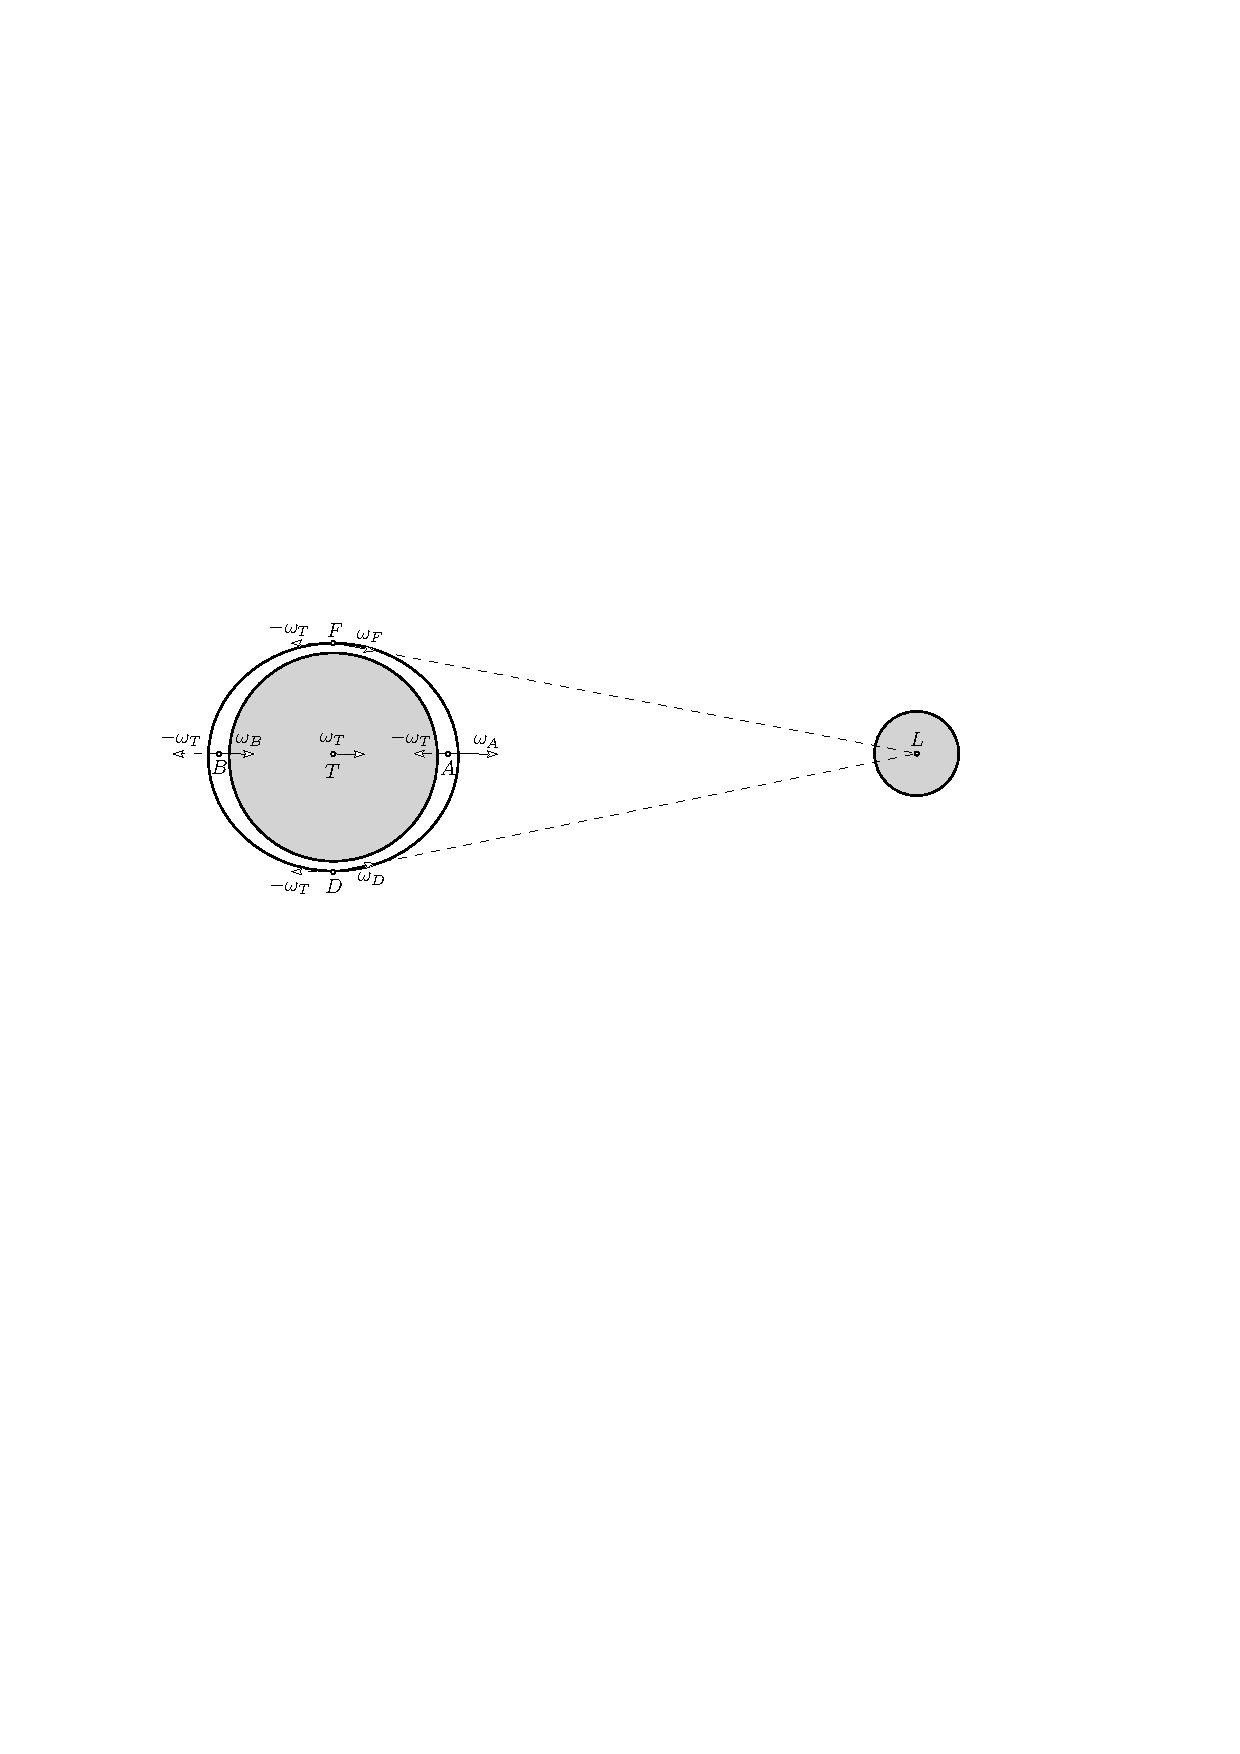
\includegraphics[width = 0.74\tw]{Ebb_flow}
    \caption{К объяснению приливных сил}\label{Ebb_flow}
\end{wrapfigure}
Ускорение в центре Земли ($T$) определяется формулой \eqref{eq:g}:
\begin{equation*}
    a_T=\frac{G M}{r^2},
\end{equation*}
где $M$~--- масса возмущающего тела, $r$~--- расстояние между центрами Земли и данного тела. Аналогично, ускорения в точках $A$ и $B$ равны соответственно
\begin{equation}
    a_A = \frac{G M}{(r - R)^2} \quad \text{и} \quad a_B = \frac{GM}{(r + R)^2},
\end{equation}
где $R$~--- радиус Земли или иного тела, подверженного воздействию приливных сил. Ускорение в точке $A$ относительно точки $T$ равно
\begin{equation}
    a_A - a_T = GM \cdot \frac{r^2 - (r - R)^2}{r^2 (r - R)^2} \xrightarrow{R \ll r} \frac{2 G M R}{r^3}.
    \label{eq:ebb-force}
\end{equation}

Под действием лунного притяжения водная оболочка Земли принимает форму
эллипсоида, который вытянут по направлению к Луне. Близ точек $A$ и $B$ будет
прилив, а в точках $F$ и $D$ --- отлив (см.~Рис.\,\ref{Ebb_flow}).

Если расстояние между телами будет достаточно мало, то одно из них из них может начать разрушаться вследствие приливных сил.

\term{Предел Роша}~--- радиус круговой орбиты спутника, обращающегося вокруг небесного тела, на котором приливные силы, вызванные гравитацией центрального тела, равны собственной силе гравицации спутника. На расстоянии равному пределу Роша любое малое возмущение на поверхности меньшего тела приведёт к его разрушению. Для того чтобы его найти требуется приравнять выражение для приливной силы (\ref{eq:ebb-force}) к ускорению свободного падения $g$ на поверхности спутника:
\begin{equation*}
    g=\frac{G m}{R^2}=\frac{4}{3} \pi G \rho_{\text{s}} R
\end{equation*}
Отсюда можно получить предел Роша:
\begin{equation*}
    r_{\text{crit}} = \sqrt[3]{\frac{3M}{2\pi\rho_{\text{s}}}}=R_{\text{c}} \sqrt[3]{\frac{2\rho_{\text{c}}}{\rho_{\text{s}}}}
\end{equation*}
Где $M, R_{\text{c}}, \rho_{\text{c}}$~--- соответствующие параметры центрального (возмущающего) тела и $\rho_{\text{s}}$~--- плотность спутника. Стоит отметить, что тут рассматривается случай твёрдого спутника, в случае жидкого спутника предел Роша возрастает примерно в два раза.
